\documentclass[sigconf]{acmart}
\usepackage{tabulary}
\usepackage{booktabs}
%%
%% \BibTeX command to typeset BibTeX logo in the docs
\AtBeginDocument{%
  \providecommand\BibTeX{{%
    Bib\TeX}}}

%% Rights management information.  This information is sent to you
%% when you complete the rights form.  These commands have SAMPLE
%% values in them; it is your responsibility as an author to replace
%% the commands and values with those provided to you when you
%% complete the rights form.
\setcopyright{none}
\copyrightyear{2024}
\acmYear{2024}
\acmDOI{XXXXXXX.XXXXXXX}

%% These commands are for a PROCEEDINGS abstract or paper.
\acmConference[Data Mining Project '24]{Data Mining Project}{April 2024}{Boulder, CO}
%%
%%  Uncomment \acmBooktitle if the title of the proceedings is different
%%  from ``Proceedings of ...''!
%%
%%\acmBooktitle{Woodstock '18: ACM Symposium on Neural Gaze Detection,
%%  June 03--05, 2018, Woodstock, NY}
%% \acmISBN{978-1-4503-XXXX-X/18/06}

%%
%% Submission ID.
%% Use this when submitting an article to a sponsored event. You'll
%% receive a unique submission ID from the organizers
%% of the event, and this ID should be used as the parameter to this command.
%%\acmSubmissionID{123-A56-BU3}

%%
%% For managing citations, it is recommended to use bibliography
%% files in BibTeX format.
%%
%% You can then either use BibTeX with the ACM-Reference-Format style,
%% or BibLaTeX with the acmnumeric or acmauthoryear sytles, that include
%% support for advanced citation of software artefact from the
%% biblatex-software package, also separately available on CTAN.
%%
%% Look at the sample-*-biblatex.tex files for templates showcasing
%% the biblatex styles.
%%

%%
%% The majority of ACM publications use numbered citations and
%% references.  The command \citestyle{authoryear} switches to the
%% "author year" style.
%%
%% If you are preparing content for an event
%% sponsored by ACM SIGGRAPH, you must use the "author year" style of
%% citations and references.
%% Uncommenting
%% the next command will enable that style.
%%\citestyle{acmauthoryear}


%%
%% end of the preamble, start of the body of the document source.
\begin{document}

%%
%% The "title" command has an optional parameter,
%% allowing the author to define a "short title" to be used in page headers.
\title{Energy Grid Forecasting and Anomaly Detection}

%%
%% The "author" command and its associated commands are used to define
%% the authors and their affiliations.
%% Of note is the shared affiliation of the first two authors, and the
%% "authornote" and "authornotemark" commands
%% used to denote shared contribution to the research.

\author{Cody Hill}
\affiliation{%
  \institution{University of Colorado Boulder}
  \city{Boulder}
  \country{USA}}
\email{cody.hill-1@colorado.edu}


%%
%% By default, the full list of authors will be used in the page
%% headers. Often, this list is too long, and will overlap
%% other information printed in the page headers. This command allows
%% the author to define a more concise list
%% of authors' names for this purpose.
\renewcommand{\shortauthors}{C. Hill et al.}

%%
%% The abstract is a short summary of the work to be presented in the
%% article.
\begin{abstract}
Energy forecasting is a vital part of today's energy markets and operations. It is used to set the cost of electricity, determine when power generation should be increased, or decide when power needs to be directed to or from other regions of the electrical grid. Electrical energy demand continues to rise, especially with the recent widespread adoption of electric vehicles. As a result, the electrical grid will need to become more robust and adaptive as this transition away from fossil fuels and into a more diversified energy market occurs. This makes forecasting predictions of electrical loads and generation that much more important and it is necessary to research the differences in forecasting applications and relevance in various short-term, medium-term, and long-term settings.

The time series forecasting techniques in use today each have their own strengths and weaknesses. Autoregressive Integrated Moving Average (ARIMA) and Exponential Smoothing models tend to be useful in short-term forecasts, but machine learning techniques such as Gradient Boosting Machines or XGBoost and Long Short-Term Memory (LSTM) network models tend to excel at longer-term forecasts. By evaluating each forecasting technique's accuracy across various context windows and forecasting horizons, the results show which techniques are most relevant within the energy grid context and for what application domain.
\end{abstract}

%%
%% The code below is generated by the tool at http://dl.acm.org/ccs.cfm.
%% Please copy and paste the code instead of the example below.
%%
\begin{CCSXML}
<ccs2012>
   <concept>
       <concept_id>10002950.10003648.10003688.10003693</concept_id>
       <concept_desc>Mathematics of computing~Time series analysis</concept_desc>
       <concept_significance>500</concept_significance>
       </concept>
   <concept>
       <concept_id>10010147.10010257.10010258.10010259.10010264</concept_id>
       <concept_desc>Computing methodologies~Supervised learning by regression</concept_desc>
       <concept_significance>500</concept_significance>
       </concept>
   <concept>
       <concept_id>10010147.10010257.10010293.10003660</concept_id>
       <concept_desc>Computing methodologies~Classification and regression trees</concept_desc>
       <concept_significance>300</concept_significance>
       </concept>
   <concept>
       <concept_id>10010147.10010257.10010293.10010075.10010295</concept_id>
       <concept_desc>Computing methodologies~Support vector machines</concept_desc>
       <concept_significance>300</concept_significance>
       </concept>
   <concept>
       <concept_id>10010147.10010257.10010293.10010294</concept_id>
       <concept_desc>Computing methodologies~Neural networks</concept_desc>
       <concept_significance>300</concept_significance>
       </concept>
   <concept>
       <concept_id>10010405.10010481.10010487</concept_id>
       <concept_desc>Applied computing~Forecasting</concept_desc>
       <concept_significance>500</concept_significance>
       </concept>
 </ccs2012>
\end{CCSXML}

\ccsdesc[500]{Mathematics of computing~Time series analysis}
\ccsdesc[500]{Computing methodologies~Supervised learning by regression}
\ccsdesc[300]{Computing methodologies~Classification and regression trees}
\ccsdesc[300]{Computing methodologies~Support vector machines}
\ccsdesc[300]{Computing methodologies~Neural networks}
\ccsdesc[500]{Applied computing~Forecasting}

%%
%% Keywords. The author(s) should pick words that accurately describe
%% the work being presented. Separate the keywords with commas.
\keywords{time series forecasting, anomaly detection, energy load, renewables, energy grid}
%% A "teaser" image appears between the author and affiliation
%% information and the body of the document, and typically spans the
%% page.
\begin{teaserfigure}
  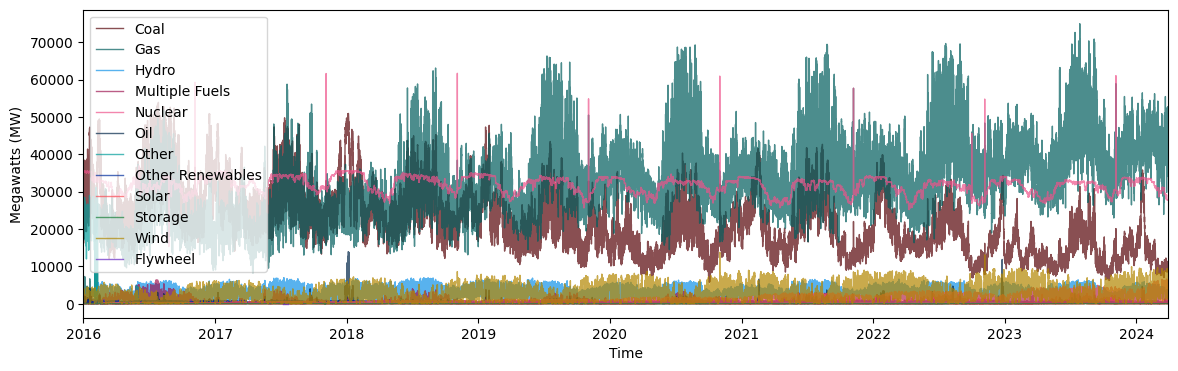
\includegraphics[width=\textwidth]{Images/Energy_Gen_Teaser.png}
  \caption{Energy Generated in megawatts (MW) by Fuel Type.}
  \Description{}
  \label{fig:teaser}
\end{teaserfigure}

%%
%% This command processes the author and affiliation and title
%% information and builds the first part of the formatted document.
\maketitle

\section{Introduction}
Energy forecasting is an important task to not only determine the expected load on the energy grid and the requirements of energy providers to meet that demand by either ramping up production or diverting sources altogether. Identifying hourly, daily, and seasonal energy demands accurately has huge implications on not only the infrastructure of our energy grid but also a complex energy marketplace where prices dynamically shift based on generation supply, customer demand, and financial spot and derivative contracts which are based on energy forecasting.[x] In the past this predictive role was largely upheld with statistical point-estimate models, but with the growth of our predictive models along with the diversification of the energy grid more modern probabilistic interval forecasting techniques have begun to be used.[x] This diversification of the energy grid not only comes from a dismantling of the monopolistic qualities of the energy market in the 1990's,[x] but emerging cultural desires and improved technology in renewable energies are driving a need for a better electrical grid.[x] 

Electricity generation has always been mostly an on-demand industry and largely continues to be, where the energy we generate needs to be transmitted in used within a short period of time because we lack efficient systems for energy storage at scale.[x] This fact presents additional complications when the majority of renewable energies only work in certain conditions, making its effective use more reliant on forecasting than traditional energy generation technologies. However, this means with accurate forecasting, we can reduce reliance on fossil-fuel energies by more efficiently filling in gaps of energy demands with renewables.

\begin{table}
\centering
\caption{Defining prediction forecast horizons. The forecast horizon determines how far into the future a forecast model predicts.}
\begin{tabular}{clc}
\toprule
\hfill No. & \hfil Forecast Horizon Intervals & Duration\\
\cmidrule(lr){1-1}\cmidrule(rl){2-2}\cmidrule(rl){3-3}
  1 & Very Short-Term & $ X < $ 1 Hour \\
  2 & Short-Term  & 1 Hour $ \leq X < $ 1 Week  \\   
  3 & Medium-Term & 1 Week $ < X \leq $ 1 Year  \\   
  4 & Long-Term & $ X > $ 1 Year  \\ 
  \bottomrule
\end{tabular}
\end{table}

\section{Related Work}
PLACEHOLDER

\section{Proposed Work}
Models stemming from different statistical and machine-learning families will be trained to perform electricity load forecasting on the forecast horizons listed in Table 1. Each model's amount of compute required for training and evaluation scores will be compared on different forecast horizons. See evaluation section for more details on the specific metrics used.

  \subsection{Data}
  Data was collected by the Pennsylvania-New Jersey-Maryland Interconnection (PJM). PJM is a regional electrical transmission organization which coordinates electricity transmission in all or parts of Delaware, Illinois, Indiana, Kentucky, Maryland, Michigan, New Jersey, North Carolina, Ohio, Pennsylvania, Tennessee, Virginia, West Virginia and the District of Columbia.[x] 
  
  Two sources of data from PJM are being utilized here, hourly load in megawatt-hours verified by the individual electric distribution companies and hourly electrical generation aggregated by fuel type, also in megawatts. The hourly load data is flagged with geographical location data which will be leveraged to include regional weather data as a covariate in the models.
  
  \subsection{Tools and Techniques}
  First these three datasets will be datetime aligned and analyzed for an outliers. The different generation sources and load data will then be analyzed and plotted for historical trends and to identify periodicity (cycles) at different context window intervals which will help set expected baselines for the forecast horizons. Once the data has been properly aggregating and aligned the data will then be split into a training, validation, and test split [METHOD TBD].

Models of varying complexity and methodology will be used to better represent the broad spectrum of techniques used today, and to attempt to capture a good representation of which models work best for the different forecast horizons. 

\textbf{Proposed models}:
\\
Baseline
\begin{itemize}
    \item{Naive Forecast Model}
\end{itemize}
Statistical
\begin{itemize}
    \item{Autoregressive Integrated Moving Average (ARIMA)}
    \item{Vector Autoregression (VAR)}
\end{itemize}
Machine Learning
\begin{itemize}
    \item{Support Vector Machine (SVM)}
    \item{XGBoost}
\end{itemize}
Deep Learning
\begin{itemize}
    \item{Long Short-Term Memory (LSTM) Networks}
    \item{Transformer Networks}
\end{itemize}
Pre-trained
\begin{itemize}
    \item{Time Series to Vector (TS2Vec)}
\end{itemize}

\section{Evaluation}
PLACEHOLDER

\section{Discussion}
PLACEHOLDER

\section{Conclusion}
PLACEHOLDER

\section{Appendices}
PLACEHOLDER

If your work needs an appendix, add it before the
``\verb|\end{document}|'' command at the conclusion of your source
document.

Start the appendix with the ``\verb|appendix|'' command:
\begin{verbatim}
  \appendix
\end{verbatim}
and note that in the appendix, sections are lettered, not
numbered. This document has two appendices, demonstrating the section
and subsection identification method.


%%
%% The acknowledgments section is defined using the "acks" environment
%% (and NOT an unnumbered section). This ensures the proper
%% identification of the section in the article metadata, and the
%% consistent spelling of the heading.
\begin{acks}
To Robert, for the bagels and explaining CMYK and color spaces.
\end{acks}

%%
%% The next two lines define the bibliography style to be used, and
%% the bibliography file.
\bibliographystyle{ACM-Reference-Format}
\bibliography{references}


%%
%% If your work has an appendix, this is the place to put it.
\appendix

\section{Research Methods}

\subsection{Part One}

Lorem ipsum dolor sit amet, consectetur adipiscing elit. Morbi
malesuada, quam in pulvinar varius, metus nunc fermentum urna, id
sollicitudin purus odio sit amet enim. Aliquam ullamcorper eu ipsum
vel mollis. Curabitur quis dictum nisl. Phasellus vel semper risus, et
lacinia dolor. Integer ultricies commodo sem nec semper.

\subsection{Part Two}

Etiam commodo feugiat nisl pulvinar pellentesque. Etiam auctor sodales
ligula, non varius nibh pulvinar semper. Suspendisse nec lectus non
ipsum convallis congue hendrerit vitae sapien. Donec at laoreet
eros. Vivamus non purus placerat, scelerisque diam eu, cursus
ante. Etiam aliquam tortor auctor efficitur mattis.

\section{Online Resources}

Nam id fermentum dui. Suspendisse sagittis tortor a nulla mollis, in
pulvinar ex pretium. Sed interdum orci quis metus euismod, et sagittis
enim maximus. Vestibulum gravida massa ut felis suscipit
congue. Quisque mattis elit a risus ultrices commodo venenatis eget
dui. Etiam sagittis eleifend elementum.

Nam interdum magna at lectus dignissim, ac dignissim lorem
rhoncus. Maecenas eu arcu ac neque placerat aliquam. Nunc pulvinar
massa et mattis lacinia.

\end{document}
\endinput
%%
%% End of file `sample-sigconf.tex'.
